\documentclass[a4paper]{scrartcl}                        % Blatt
\usepackage[left=3cm,right=3cm,top=3cm,bottom=4cm]{geometry}    % Ränder
\usepackage{amsmath,amsthm,amssymb,mathtools}                   % Mathestuff
\usepackage{physics,mathptmx,siunitx,isotope}                   % Matheformat Stuff
\usepackage[utf8]{inputenc}                                     % lässt dich nativ ä ß etc. eingeben
\usepackage[ngerman]{babel}                                     % macht zeugs deutsch
\usepackage{booktabs,url,caption}                               % quality of life packages in speziellen Situationen
\usepackage{lmodern,wrapfig}

% stellt ein, wie SI deine Einheiten formatiert
% kann man jederzeit geändert vor sein Zeugs kopieren, dann wird das ab da genutzt
\sisetup{scientific-notation=engineering, exponent-product = \cdot, output-decimal-marker = {,}, separate-uncertainty, exponent-to-prefix}
\DeclareCaptionType{Liste}[Liste][Liste]                        % von caption, lässt dich andere Sachen als Abb. und Tab. definieren

\begingroup                                                     %
\catcode`_=\active                                              % fancy shit
\gdef\enablesbsb{                                               % müsst ihr nich verstehen
   \catcode`_=\active                                           % vertsteh ich btw auch nich
   \def_##1{\ifx_##1\expandafter\sbtext\else\sb{##1}\fi}        %
}                                                               % lässt euch
\gdef\disablesbsb{\catcode`_=8}                                 % a_x & a_{xx} für Mathesymbolindices &
\endgroup                                                       % a__x & a__{xx} für Text machen!
\def\sbtext#1{\sb{\text{#1}}}                                   % Bitte nutzt das

\newcommand{\imu}{\mathrm{i}}

\begin{document}
\enablesbsb % macht a__x an

\section{Wechselstromkreise}
\Large 
\begin{frame}
    \centering
    \visible<2->{
    \begin{tikzpicture}
        \path[very thick, -{Latex}] (0, 0) edge (10, 0) (0, -1) edge (0, 3);
        \node[right] at (10, 0) {$t$};
        \draw[thick, red] (0, 0) sin (1, 1) cos (2, 0)
            sin (3, -1) cos (4, 0)
            sin (5, +1) cos (6, 0)
            sin (7, -1) cos (8, 0);
    \end{tikzpicture}
    }
    \\
    \visible<3>{
        \[ A(t) = \hat A\sin(\omega t + \phi) \]
    }
\end{frame}

\section{Die Bauteile}
\begin{frame}
    \centering\Huge
    \visible<1->{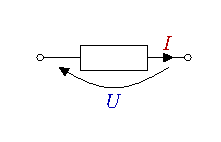
\includegraphics[width=.5\textwidth]{../script/kBR.pdf}}
    \visible<2->{
    \parbox[b]{.4\textwidth}{
        $$U = R\cdot I$$
        \vspace{16mm}
    }}
    \vspace{-1cm}  % caught in the act
    \visible<3>{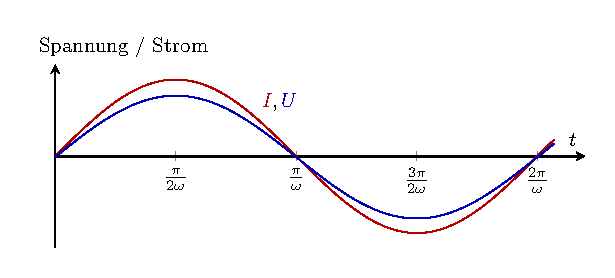
\includegraphics[width=.7\textwidth]{../script/kPR.pdf}}
\end{frame}
\begin{frame}
    \centering\huge
    \visible<1->{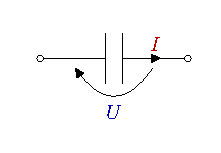
\includegraphics[width=.5\textwidth]{../script/kBC.pdf}}
    \visible<2->{
    \parbox[b]{.4\textwidth}{
        $$I = C\dot U$$
        \vspace{16mm}
    }}
    \visible<3>{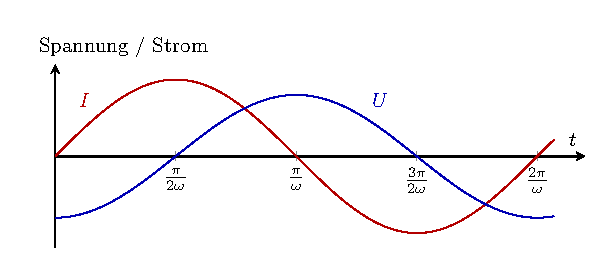
\includegraphics[width=.7\textwidth]{../script/kPC.pdf}}
\end{frame}
\begin{frame}
    \centering\huge
    \visible<1->{\includegraphics[width=.5\textwidth]{../script/kBL.pdf}}
    \visible<2->{
    \parbox[b]{.4\textwidth}{
        $$U = L\dot I$$
        \vspace{16mm}
    }}
    \vspace{-1cm}  % caught in the act
    \visible<3>{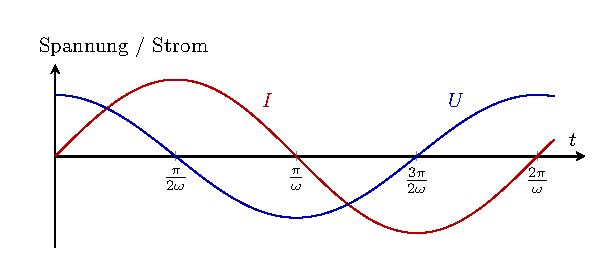
\includegraphics[width=.7\textwidth]{../script/kPL.pdf}}
\end{frame}

\subsection{Komplexe Zahlen}
Normalerweise werden komplexe Zahlen via der imaginären Einheit $\imu^2 \coloneqq -1$ eingeführt.
Anschließend definiert man dann die komplexen Zahlen über $\mathbb{C} \ni c \coloneqq a + b\cdot \imu$ mit $a,b \in \mathbb{R}$.
Aus dieser Herangehensweise folgen dann recht schnell die Regeln zum Rechnen mit ebendiesen.
\begin{align*}
    c_1 +c_2 &= (a_1 + b_1\cdot \imu) + (a_2 + b_2\cdot \imu) &
    c_1 \cdot c_2 &= (a_1 + b_1\cdot \imu) \cdot (a_2 + b_2\cdot \imu) \\
        &= (a_1 + a_2) + (b_1 + b_2)\cdot \imu  &
        &= a_1a_2 + b_1b_2 \cdot \imu^2 + a_1b_2 \cdot \imu + a_2b_1 \cdot \imu\\
        &&&= (a_1a_2 - b_1b_2) + (a_1b_2 + a_1b_2) \cdot \imu
\end{align*}

\begin{wrapfigure}{r}{0.4\textwidth}
  \begin{centering}
    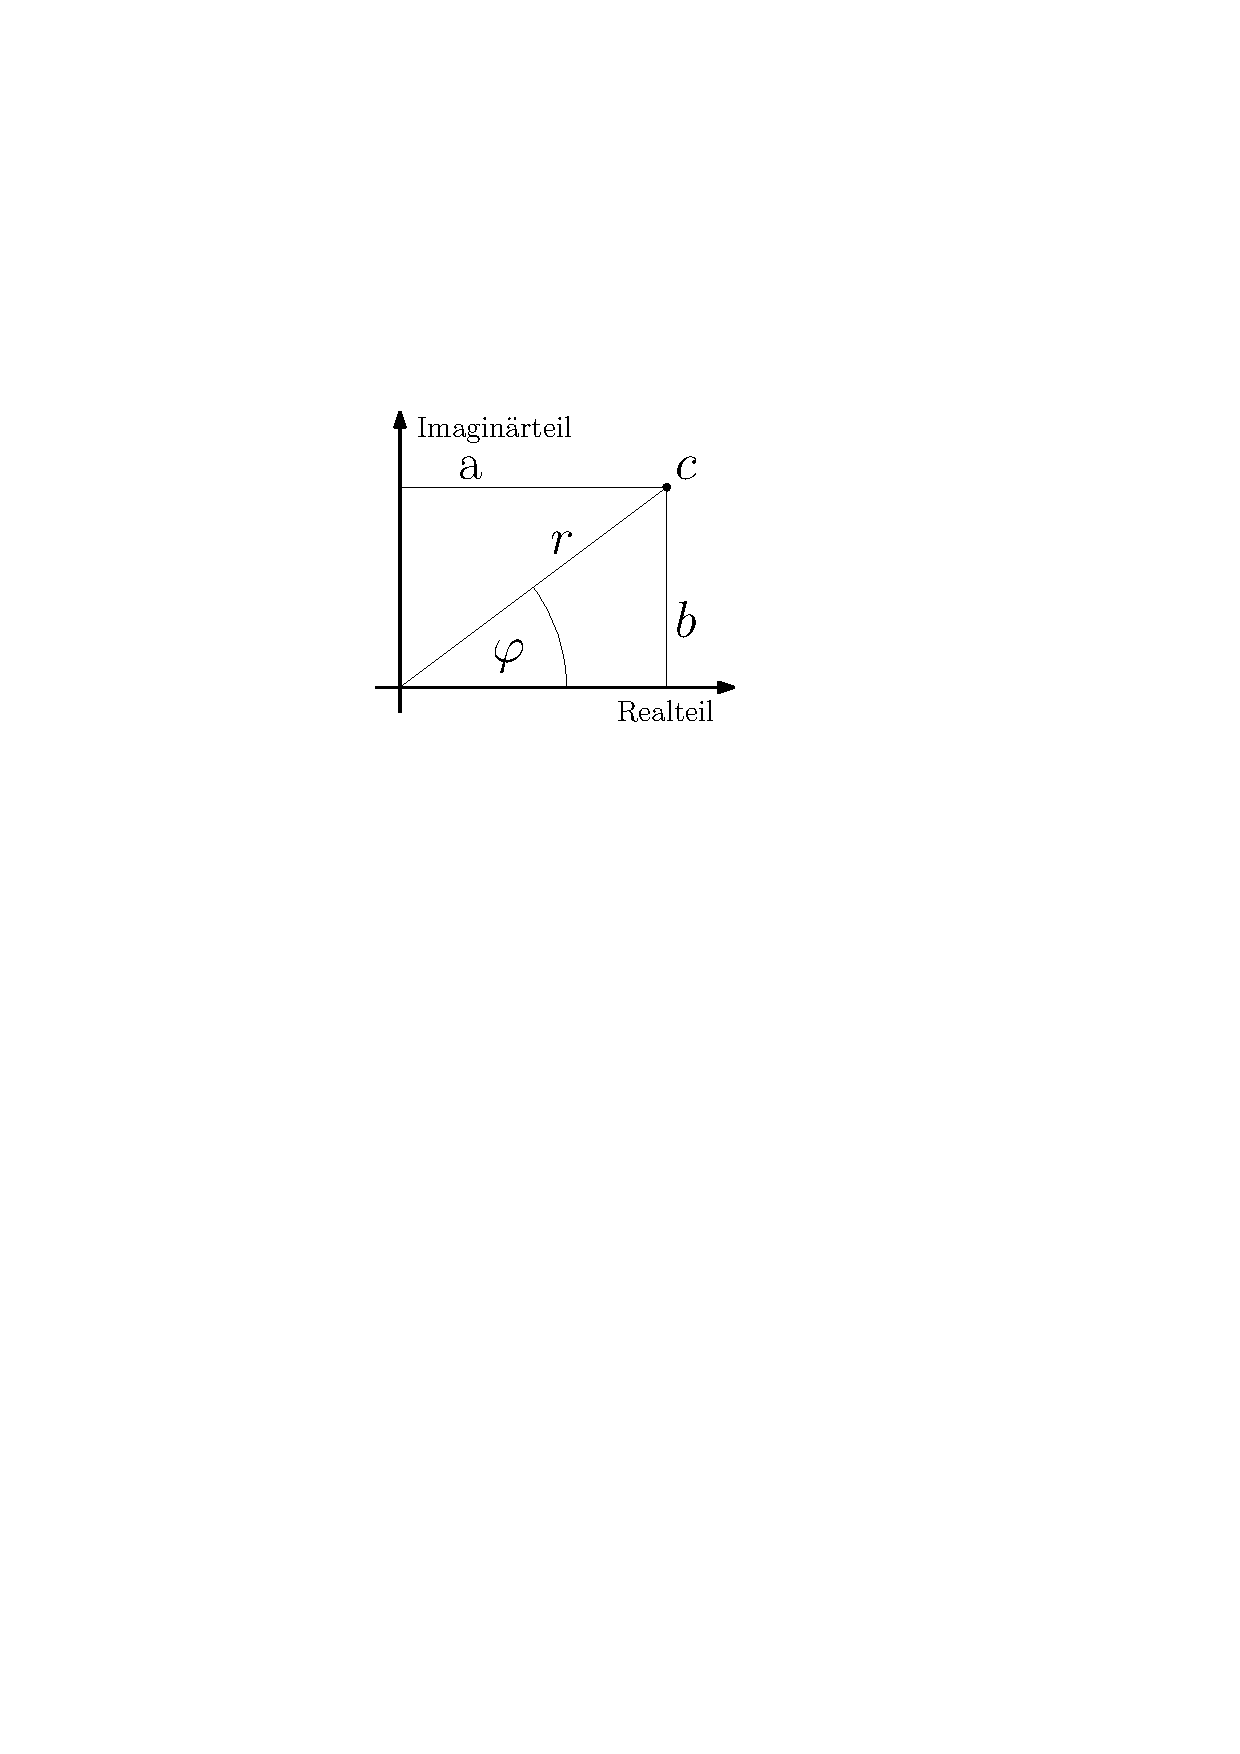
\includegraphics[width=0.4\textwidth]{philip1.pdf}
  \end{centering}
  \caption{Komplexe Zahl $c$ in kartesischen und polaren Koordinaten}
\end{wrapfigure}

Für den Anwendungsbereich der Wechselstromberechnungen ist es jedoch sinnvoller, komplexe Zahlen als
Repräsentanten von Punkten im zweidimensionalen Raum zu sehen, welche über die oben genannten Rechenvorschriften nützliche Eigenschaften besitzen, auf die im folgenden eingegangen werden soll.

Man denke sich eine komplexe Zahl $a +b\imu$ als einen Vektor $(a,\,b)_{x,y}$ im kartesischen Koordinatensystem mit X- und Y-Achse.
Dann sieht man, dass die Addition zweier komplexer Zahlen genau der Vektoraddition entspricht.
Weiterhin kann man den Vektor auch in einem polaren Koordinatensystem darstellen, in dem man aus $a$ und $b$ den 
Abstand zum Koordinatenursprung $r$ und den Winkel zur X-Achse $\varphi$ berechnet. Diese Form führt zu einer deutlich einprägsameren Multiplikationsformel.  
\begin{align*}
    a&=r \cdot \cos(\varphi) & c_1 &= a_1+b_1\imu = r_1\cos(\varphi_1) + r_1\sin(\varphi_1)\imu  \\
    b&=r \cdot \sin(\varphi) & c_2 &= a_2+b_2\imu = r_2\cos(\varphi_2) + r_2\sin(\varphi_2)\imu
\end{align*} \vspace*{-5mm}
\begin{align*}
    c_1 \cdot c_2 &= (r_1r_2\cos(\varphi_1)\cos(\varphi_2) - r_1r_2\sin(\varphi_1)\sin(\varphi_2)) \\
    &\quad + (r_1r_2\cos(\varphi_1)\sin(\varphi_2) + r_1r_2\cos(\varphi_2)\sin(\varphi_1)) \cdot \imu\\
    &= r_1r_2 \cdot \big(\cos(\varphi_1 + \varphi_2) + \sin(\varphi_1 + \varphi_2)\imu\, \big)
\end{align*} \vspace*{-5mm}
\begin{align*}
    (r_1,\varphi_1)_{r,\,\varphi} \cdot (r_2,\,\varphi_2)_{r,\varphi} = (r_1 \cdot r_2,\, \varphi_1 + \varphi_2)_{r,\varphi}
\end{align*}
Die Multiplikation zweier solcher Vektoren dreht den ersten also noch um den Winkel des zweiten weiter, und streckt die Länge $r_1$ um den Faktor $r_2$

\section{Verhaltensdarstellung über Komplexe Zahlen}

Um nun zu verstehen, wie komplexe Zahlen nun hilfreich sein können,
um die Interaktion von passiven elektrischen Bauteilen mit dem eingehenden Spannungs- oder Stromsignal 
zu berechnen, benötigt man ein Verständnis der Multiplikation komplexer Zahlen in der Polardarstellung.


\begin{align*}
    Z_1&= (r_1, \varphi_1) & Z_1 \cdot Z_2 = (r_1 \cdot r_2, \varphi_1 + \varphi_2) \\
    Z_2&= (r_2, \varphi_2)
\end{align*}

\subsection{Signal}
Eine kreisförmige Schwingung um den Ursprung lässt sich nun

\subsection{Impendanz}
This is more testing text.


\end{document}
